%Main Document
\documentclass[a4paper, 11pt, oneside]{AuProjectHandin}
\usepackage{AuPreamble}
%configurationfile


\title{Dokumentation}
%author will mostly not be used unless we are talking solo work and then group members should be disabled ;)
\author{Forfatter Navn}
%Vejlederens navn
\SetVejleder{Søren}
%Skole/Universitetets navn
\SetUniversity{Aarhus Universitet}
%Projektnavn
\SetProject{Semesterprojekt 3. Semester}
%Gruppe Nummer
\SetGroupNumber{10}
%Add the names of all the members in the group, can handle 1 to 8 members, names are added one per set of []
\GroupMemberNames[Tonni Follmann][Stefan Nielsen][Mikkel Busk][Halfdan][Ahmad][Jacob]{}
%add student numbers of the students, must have the exact same order as the names listed above.
\GroupMemberStudentNo[201504573][201508282][33333][0][0][0]{}
\begin{document}

\frontmatter
\tableofcontents
%generate  table of content etc here
\mainmatter
%include content sections here
%\chapter{Dummy chapter}

Some intro text here
\section{Gruppemedlemmer}
\PrintGroupMembers
\section{section test 1}
\subsection{ sub section test 1}
blabla lafjkladjfla jfaælskjadlfa
\subsubsection{ subsubsection test }
text in the sub section blabla	
\chapter{Indledning}
\section{Projektformulering}
Mange ældre har i dag svært ved at åbne deres vinflaske, da de ikke har den fornødne styrke til selv at trække korkproppen ud af vinflasken. Derfor ville det være ideelt for dem, at have en løsning hvor åbningen af vinflaskerne bliver automatiseret.

For at få den optimale oplevelse ud af en vin, skal den åbnes rettidigt så den iltes før indtagelse. Iltningstiden kan variere fra vin til vin, og derfor kan mange uerfarne vindrikkere have svært ved at ilte deres vin korrekt. Mange glemmer at åbne vinen i god tid, og opnår derfor ikke den optimale oplevelse. Det kan derfor være ideelt, hvis denne proces også automatiseres.

\subsection{Projektdefinition}
Ud fra ovenstående problemstillinger skal der fremstilles et produkt som skal automatisere vinåbning og iltning, samt hvis muligt  oprette et netværk hvor vindrikkere og forhandlere kan sættes i forbindelse med hinanden. Produktet har følgende systemkrav:

Systemet: \begin{itemize}
	\item Skal trække korkproppen ud af en vinflaske, og ilte vinen korrekt. I denne proces indgår aktuator, sensor, PSoC, Devkit og motor.
	\item Skal betjenes via Devkit 8000, hvor der er installeret Linux.
	\item Skal meddele brugeren når vinen er klar.
	\item Skal kunne indstilles til at trække korkproppen ud til et givent tidspunkt.
	\item Skal holde vinflasken fast under udtrækningen af korkproppen.
	\item Skal detektere afstanden fra toppen af flasken til åbningsmekanismen.
	Skal kunne bortskaffe vinpropper efter åbning.
	\item Skal kunne give status for vinåbningsprocessen.
	\item Skal kunne åbne vin hurtigt, når situation kræver det.
	\item Skal have et grafisk brugerinterface til betjening af vinåbningen.
	\item Skal give brugeren mulighed for at indstille klokken på et indbygget realtidsur.
	\item Skal have et grafisk brugerinterface til betjening af vinåbningen.
	\item Bør have en sikkerhedsmekanisme til forebyggelse af personskader.
	\item Bør ud fra vinens type kunne ilte vinen korrekt.
	\item Kunne hvis muligt måle vinflaskens temperatur.
	\item Kunne hvis muligt fjernbetjenes med en mobil applikation, således at brugeren har mulighed for at ændre på et evt. åbningstidspunkt.
	\item Kunne hvis muligt tilkobles en database med information om forskellige vine og deres iltningstid, så det er muligt at automatisere iltningsprocessen ud fra de enkelte vine.
	\item Kunne hvis muligt forbindes til et online socialt netværk, så vindrikkere kan give anmeldelser af forskellige vine.
	\item Kunne hvis muligt give bruger mulighed for at bestille vine direkte fra en forhandler.
	\item Kommer ikke til at kunne tilsluttes det danske el-net.
\end{itemize}

\begin{center}
	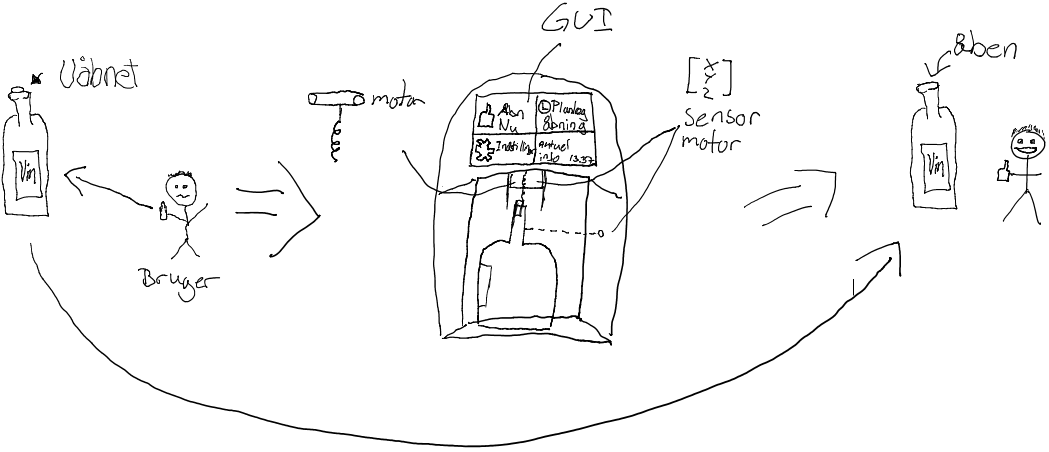
\includegraphics{WinePrep_realistisk.png}
\end{center}

\chapter{Krav}
\section{Usecase beskrivelse}
I dette afsnit vil kun de væsentligste krav blive præsenteret. Ønskes der et større indblik i beskrivelse af krav og yderligere krav til projektet henvises der til bilagsrapporten. Usecasen som er blevet udevalgt her er "Planlæg åbning", da den også indeholde alt hvad der er i usecasen "Åbn nu". "Åbn nu" usecasen kan findes under bilag x, i doukumentationen. Der er yderligere en usecase som ikke er blevet medtaget i denne rapport. Det er Usecasen "Indstil tid". Denne er ikke blevet medtaget, da den ikke har den store påvirkning på iltåbningsprocessen.

\subsection{Aktørbeskrivelse}

\paragraph{Bruger:} Brugeren er systemets primære aktør. Brugeren er ham eller hende der betjener systemet, og har en opgave som ønskes løst af systemet.

\subsection{Use-case 2: Planlæg Åbning}
Usecasen "Planlæg åbning" ser således ud:

\label{UC2}
\rowcolors{1}{white}{lightgray}
\LTXtable{360pt}{tables/UC2}
\pagebreak

%appendix, biblography, index etc here.

\section{Ikke-funktionelle krav}
Igen vil der her kun blive præsenteret de væsentligste ikke-funktionelle krav. For at se  alle ikke-funktionelle krav henvises til bilag x.
\subsection{Brugervenlighed}

\begin{enumerate}
\item Systemet skal give brugeren beskeder om vinens status via tekst på touch skærmen.
\end{enumerate}

\subsection{Ydeevne}
\begin{enumerate}
\item Når brugeren vælger "Planlæg åbning", skal systemet kunne åbne vinflaksen med en afvigelse på max 1 minut fra det indstillede åbningstidspunkt. Her skal åbning af vinen ligeledes kunne færdiggøres af systemet på max 1 minut.
\item Systemet skal kunne håndtere en vinflaske af typen x
\end{enumerate}

\subsection{Vedligeholdelse}
\begin{enumerate}
\item Motor- og sensorstyring skal foregå via en PSoC.
\end{enumerate}

\chapter{Afgrænsing}
Som udgangspunkt havde det endelige produkt mange flere funktioner end det er endt med. På baggrund af en RISK-analyse blev prioritetsrækkefølgen afgjort. Det blev besluttet at dem med højest RISK-faktor skulle være det der skulle startes på først. Derfor blev funktioner som WineBook (et socialt medie for vindeling) hurtig ned prioriteret. For at se Risk-analysen henvises til bilag x i dokementationsrapporten.


\end{document}